% RDL Figure F08 v1.0 -- conditional sign-convention map.
% Artefact status: reproducible figure candidate.
% Required packages: tikz, amsmath, lmodern.
% Required TikZ libraries: arrows.meta, positioning, fit, calc.
% Publication use: include figures/final/RDL-F08-v1.0.pdf with \includegraphics.
\documentclass[tikz,border=7pt]{standalone}
\usepackage[T1]{fontenc}
\usepackage{lmodern}
\usepackage{amsmath}
\usetikzlibrary{arrows.meta,positioning,fit,calc}

\definecolor{RDLblue}{RGB}{40,77,112}
\definecolor{RDLgreen}{RGB}{42,111,88}
\definecolor{RDLamber}{RGB}{181,113,31}
\definecolor{RDLpale}{RGB}{241,245,248}
\definecolor{RDLgray}{RGB}{93,99,105}

\tikzset{
  rdl sign/.style={
    draw=black,
    line width=0.7pt,
    rounded corners=2pt,
    fill=RDLpale,
    text width=4.15cm,
    minimum height=2.55cm,
    align=center,
    inner sep=5pt,
    font=\small
  },
  rdl source/.style={rdl sign,fill=RDLgreen!8},
  rdl flux/.style={rdl sign,fill=RDLblue!8},
  rdl arrow/.style={-{Stealth[length=2.6mm,width=1.8mm]},line width=0.85pt},
  rdl condition/.style={
    font=\sffamily\scriptsize,
    text width=3.05cm,
    align=center,
    fill=white,
    inner sep=1.5pt
  },
  rdl failure/.style={
    draw=RDLamber!85!black,
    line width=0.55pt,
    rounded corners=2pt,
    fill=RDLamber!7,
    text width=3.45cm,
    minimum height=1.05cm,
    align=center,
    inner sep=4pt,
    font=\sffamily\scriptsize
  },
  rdl failarrow/.style={-{Stealth[length=2.1mm,width=1.5mm]},line width=0.6pt,dashed,RDLamber!85!black}
}

\begin{document}
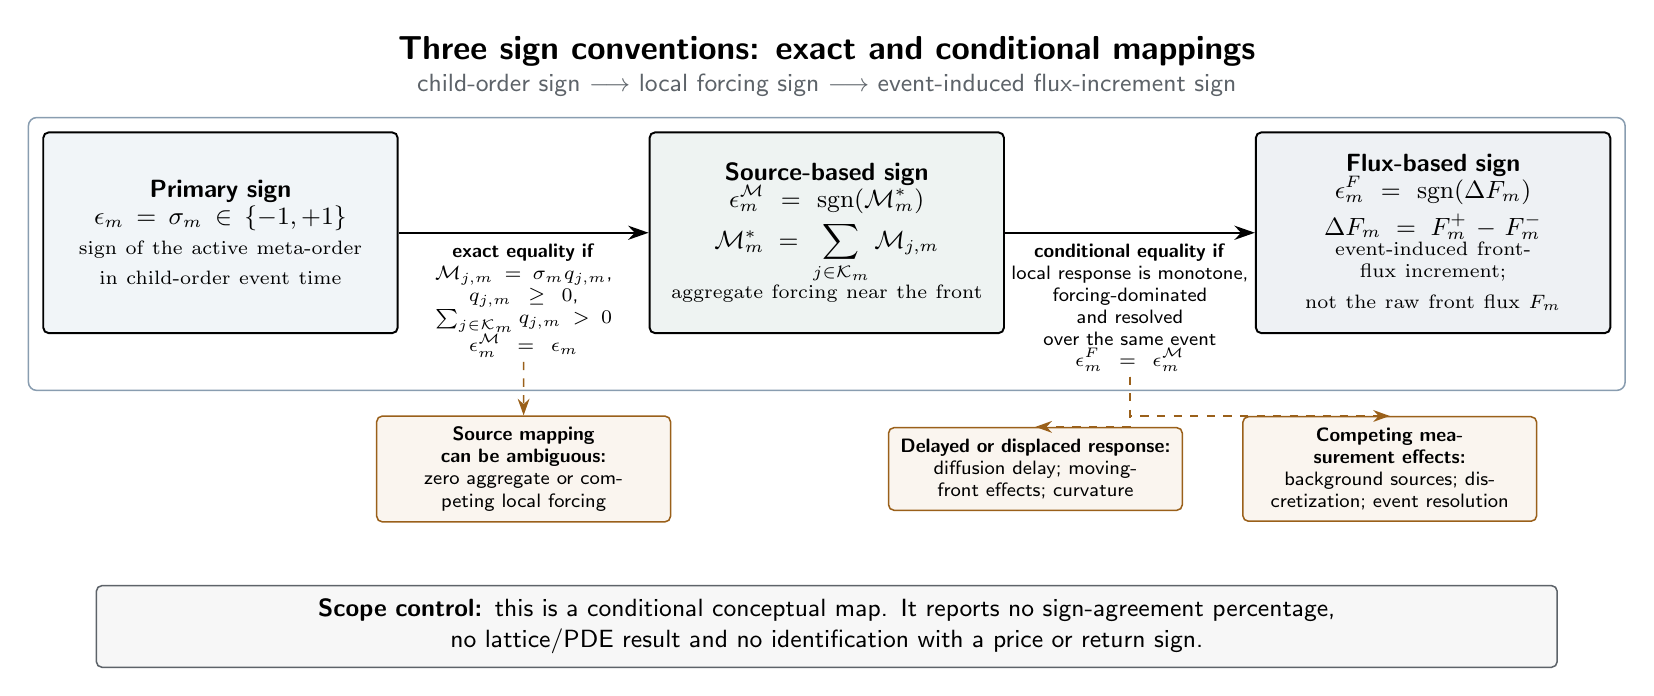
\begin{tikzpicture}[x=1cm,y=1cm]
  \node[font=\sffamily\bfseries\large] at (10.0,4.45)
    {Three sign conventions: exact and conditional mappings};
  \node[font=\sffamily\small,text=RDLgray] at (10.0,4.02)
    {child-order sign $\longrightarrow$ local forcing sign $\longrightarrow$ event-induced flux-increment sign};

  \node[rdl sign] (primary) at (2.3,2.15) {
    {\sffamily\bfseries Primary sign}\\[-0.5mm]
    $\epsilon_m=\sigma_m\in\{-1,+1\}$\\[1mm]
    {\scriptsize sign of the active meta-order\\in child-order event time}
  };

  \node[rdl source] (source) at (10.0,2.15) {
    {\sffamily\bfseries Source-based sign}\\[-0.5mm]
    $\epsilon_m^{\mathcal M}=\operatorname{sgn}(\mathcal M_m^*)$\\[0.8mm]
    $\mathcal M_m^*=\displaystyle\sum_{j\in\mathcal K_m}\mathcal M_{j,m}$\\[-0.2mm]
    {\scriptsize aggregate forcing near the front}
  };

  \node[rdl flux] (flux) at (17.7,2.15) {
    {\sffamily\bfseries Flux-based sign}\\[-0.5mm]
    $\epsilon_m^F=\operatorname{sgn}(\Delta F_m)$\\[0.8mm]
    $\Delta F_m=F_m^+-F_m^-$\\[-0.2mm]
    {\scriptsize event-induced front-flux increment;\\not the raw front flux $F_m$}
  };

  \draw[rdl arrow] (primary) -- (source);
  \node[rdl condition,anchor=north] (source-condition)
    at ($(primary.east)!0.5!(source.west)+(0,-0.08)$) {
    \textbf{exact equality if}\\
    $\mathcal M_{j,m}=\sigma_m q_{j,m}$, $q_{j,m}\geq0$,\\
    $\sum_{j\in\mathcal K_m}q_{j,m}>0$\\[-0.2mm]
    $\epsilon_m^{\mathcal M}=\epsilon_m$
  };

  \draw[rdl arrow] (source) -- (flux);
  \node[rdl condition,anchor=north] (flux-condition)
    at ($(source.east)!0.5!(flux.west)+(0,-0.08)$) {
    \textbf{conditional equality if}\\
    local response is monotone,\\
    forcing-dominated and resolved\\
    over the same event\\[-0.2mm]
    $\epsilon_m^F=\epsilon_m^{\mathcal M}$
  };

  \node[rdl failure] (fail-source) at (6.15,-0.85) {
    \textbf{Source mapping can be ambiguous:}\\
    zero aggregate or competing local forcing
  };
  \node[rdl failure] (fail-flux-a) at (12.65,-0.85) {
    \textbf{Delayed or displaced response:}\\
    diffusion delay; moving-front effects; curvature
  };
  \node[rdl failure] (fail-flux-b) at (17.15,-0.85) {
    \textbf{Competing measurement effects:}\\
    background sources; discretization; event resolution
  };

  \draw[rdl failarrow] (source-condition.south) -- (fail-source.north);
  \draw[rdl failarrow] (flux-condition.south) |- (fail-flux-a.north);
  \draw[rdl failarrow] (flux-condition.south) |- (fail-flux-b.north);

  \node[
    draw=RDLgray,
    line width=0.55pt,
    rounded corners=2pt,
    fill=black!3,
    text width=18.2cm,
    align=center,
    inner sep=5pt,
    font=\sffamily\small
  ] at (10.0,-2.85) {
    \textbf{Scope control:} this is a conditional conceptual map. It reports no
    sign-agreement percentage,\\no lattice/PDE result and no identification
    with a price or return sign.
  };

  \node[
    fit=(primary)(source)(flux)(source-condition)(flux-condition),
    rounded corners=3pt,
    draw=RDLblue!55,
    line width=0.55pt,
    inner sep=5pt
  ] {};
\end{tikzpicture}
\end{document}
